\documentclass[12pt]{article}
\usepackage{amsmath}
\usepackage{graphicx}
\usepackage{float}
\usepackage[font={small,it}]{caption}
\pagenumbering{arabic}

% This is a comment

\begin{document}
	\title{Project 1}
	\author{Michael Saybolt \\ Bjon Charlery}
	
	\date{\today}
	\maketitle
	\pagebreak
\begin{abstract}
This project explored solving differential equations, specifically \\linear second order equations, by using a couple of different methods \\ which include LU Decomposition, Gauss Forward and Backward Substitution : General algorithm
\end{abstract}
\bigskip
\bigskip
\section{Introduction}
\indent The objective of this project was to solve a differential equation in the form of:\\ $$-u\textsuperscript{''}(x) = f(x), x\epsilon(0,1),u(0) = u(1) = 0.\\$$ that can be written into the linear equation $(Ax = b)$. Since A is a tridiagonal matrix there is an actual or analytical solution that can be made for this particular matrix. The following sections will describe the origins for the algorithms used and their respective results.
\section{Description}
This section will detail the methods used to solve the linear equation system. It is solved using two methods:\\
\begin{itemize}
	\item \centering LU decomposition
	\item \centering Tridiagonal Solver - Gauss Elimination\\
\end{itemize}

\subsection{LU Decomposition Solver}
This method consists of creating a Lower-Triangular matrix $L$ and a Upper-Triangular matrix $U$ for factorizing the linear system $(A = LU)$.\\
\pagebreak
\bigskip
\bigskip
\bigskip
$$
\begin{bmatrix}
	1& 0& 0& 0& 0&\\
	l\textsubscript{21}& 1&  0& 0& 0&\\
	l\textsubscript{31}& l\textsubscript{32}& 1&  0& 0&\\
	l\textsubscript{41}& l\textsubscript{42}& l\textsubscript{43}& 1& 0&\\
	l\textsubscript{51}& l\textsubscript{52}& l\textsubscript{53}& l\textsubscript{54}& 1&
\end{bmatrix}
and
\begin{bmatrix}
1& l\textsubscript{12}& l\textsubscript{13}& l\textsubscript{14}& l\textsubscript{15}&\\
0& 1& l\textsubscript{23}& l\textsubscript{24}& l\textsubscript{25}&\\
0& 0& 1& l\textsubscript{34}& l\textsubscript{35}&\\
0& 0& 0& 1& l\textsubscript{45}& \\
0& 0& 0& 0& 1&

\end{bmatrix}
$$
Once (L) and (U) are found they can be used to solve the following equation: $(Av = LUv = h\textsuperscript{2} f)$ by allowing $(Ly = h\textsuperscript{2}f)$ and $(Uv = y)$ with backwards substitution, in this case that would be required two times.
\subsection{Tridiagonal Solver: General Gauss Elimination}
This method consists of using Gauss elimination due to the matrix (A) only having values along the three diagonals of the matrix.\\
$$
\begin{bmatrix}
b\textsubscript{1}& c\textsubscript{1}& 0& 0& ...& ...& 0&\\
a\textsubscript{1}& b\textsubscript{2}&  c\textsubscript{2}& 0& ...& ...& 0&\\
0& a\textsubscript{2}& b\textsubscript{3}&  c\textsubscript{3}& 0& ...& 0&\\
\rotatebox{90}{...}& ...& \rotatebox{320}{...}& \rotatebox{320}{...}& \rotatebox{320}{...}& ...& \rotatebox{90}{...}&\\
\rotatebox{90}{...}& ...& ...& \rotatebox{320}{...}& \rotatebox{320}{...}& \rotatebox{320}{...}& 0&\\
0& ...& ...& 0& a\textsubscript{n-1}& b\textsubscript{n-1}& c\textsubscript{n-1}&\\
0& ...& ...& ...& 0& a\textsubscript{n}& b\textsubscript{n}&
\end{bmatrix}
$$
The diagonal of the matrix will be changed using the following formula while the "Upper Diagonal" will not be changed:\\
$$d\textsubscript{i} = b\textsubscript{i} - a\textsubscript{i}c\textsubscript{i} / d\textsubscript{i-1}\\$$
The "Lower Diagonal" will be changed so that all elements below the diagonal are zeros. The vector (f) changes with the following formula:\\
$$w\textsubscript{i} = f\textsubscript{i} - a\textsubscript{i}w\textsubscript{i-1} / d\textsubscript{i-1}\\$$
With backwards substitution then can be performed after following:\\
$$v\textsubscript{i} = w\textsubscript{i-1} - c\textsubscript{i-1}v\textsubscript{i} / d\textsubscript{i-1}\\$$
\begin{centering} with $$d\textsubscript{1} = b\textsubscript{1}, w\textsubscript{1} = f \textsubscript{1}, and v\textsubscript{n} = h\textsuperscript{2}w\textsubscript{n} / d\textsubscript{n}$$
\end{centering}

\section{Results}
This section will show the overall correctness of each calculation, and the average speed of each method.
\subsection{Accuracy}
The analytical solution to f(x) = 100*exp(-10*x) is known to be u(x) = 1-(1-exp(-10))*x-exp(-10*x). This is used to compare the accuracy of the numerical solutions obtained with both the general Gaussian elimination algorithm as well as the LU decomposition version for various n.  Plots are generated to give a summarized view of the generated output files.\\

\subsection{Gauss General:}
Figure x shows the analytical solution and the numerical solution for various n using the general Gaussian elimination solver. As n increases, the result is more tightly fit to the analytical solution.\\

\begin{figure}[H]
\graphicspath{{~/GitHub/sayboltm/PHY480/Project1/Report/Precision/Gauss/} {c:/Users/charl/Documents/Precision/Gauss/}{C:/Users/Mike/Documents/GitHub/sayboltm/PHY480/Project1/Report/Precision/Gauss/}}
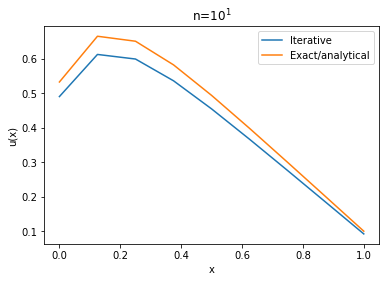
\includegraphics[scale=0.22]{1.png}
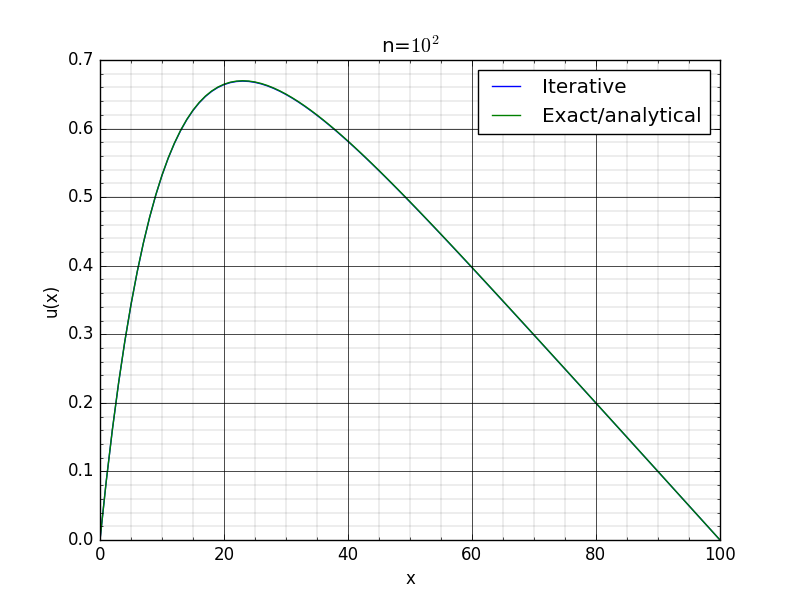
\includegraphics[scale=0.22]{2.png}
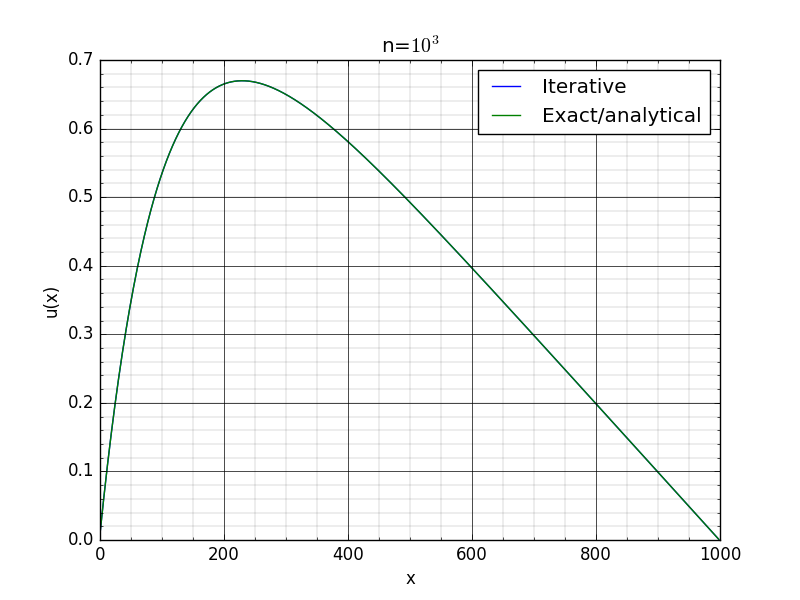
\includegraphics[scale=0.22]{3.png}
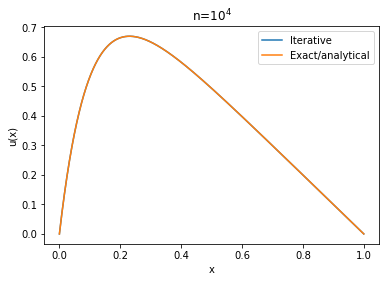
\includegraphics[scale=0.22]{4.png}
\centering
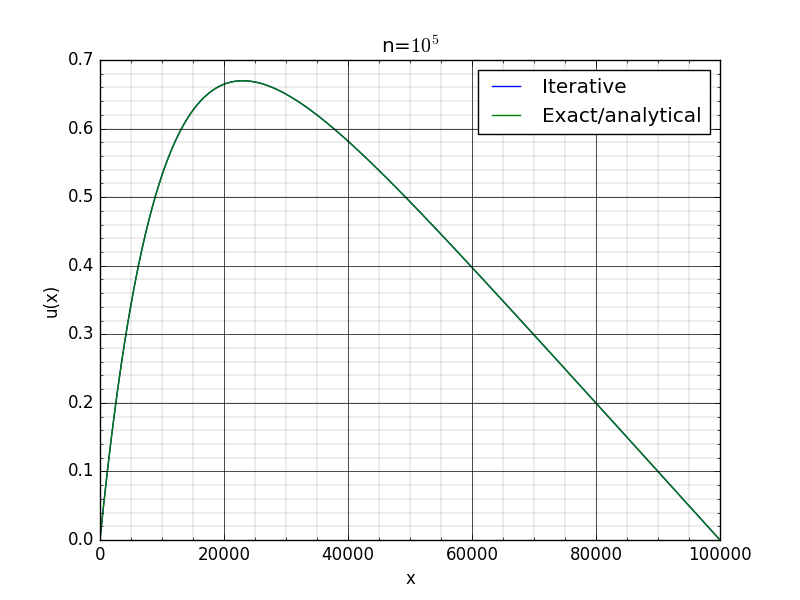
\includegraphics[scale=0.22]{5.png}\\
\centering
\caption{The relative error is computed using:
	e\textsubscript{i}=|(v\textsubscript{i}-u\textsubscript{i})/(u\textsubscript{i})
	where v\textsubscript{i} is the analytical solution value, and u\textsubscript{i} is the numerical solution value}
\end{figure}
The relative error is plotted for various n in figure y.\\
\begin{figure}[H]
\centering
\graphicspath{{~/GitHub/sayboltm/PHY480/Project1/Report/Precision/Gauss/} {c:/Users/charl/Documents/Precision/Gauss/}{C:/Users/Mike/Documents/GitHub/sayboltm/PHY480/Project1/Report/Precision/Gauss/}}
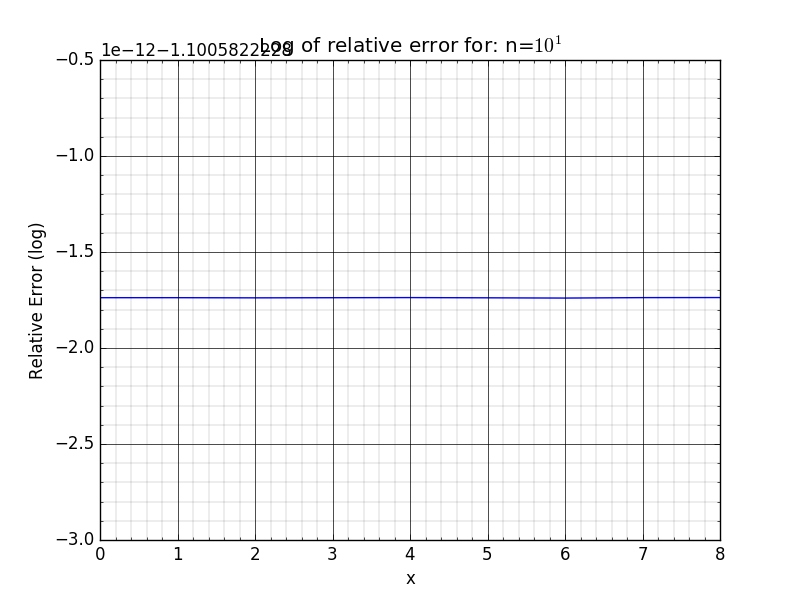
\includegraphics[scale=0.22]{1_error.png}
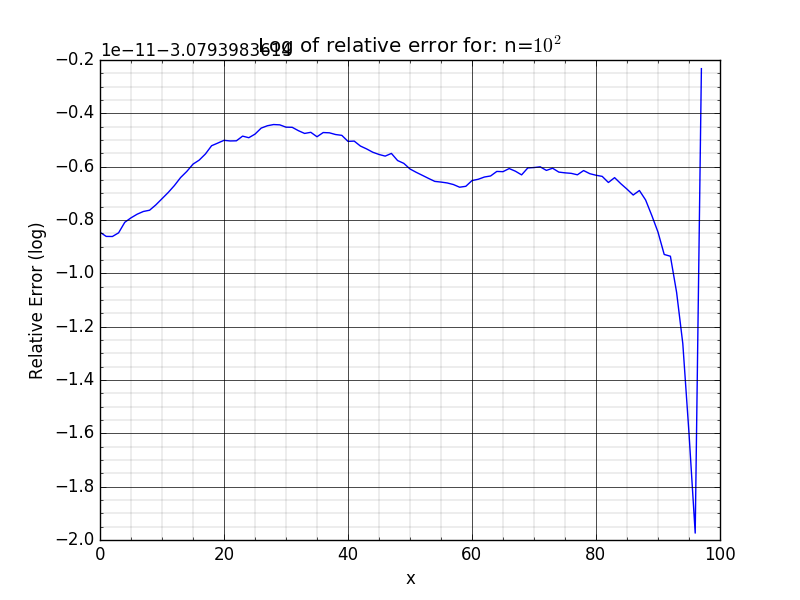
\includegraphics[scale=0.22]{2_error.png}
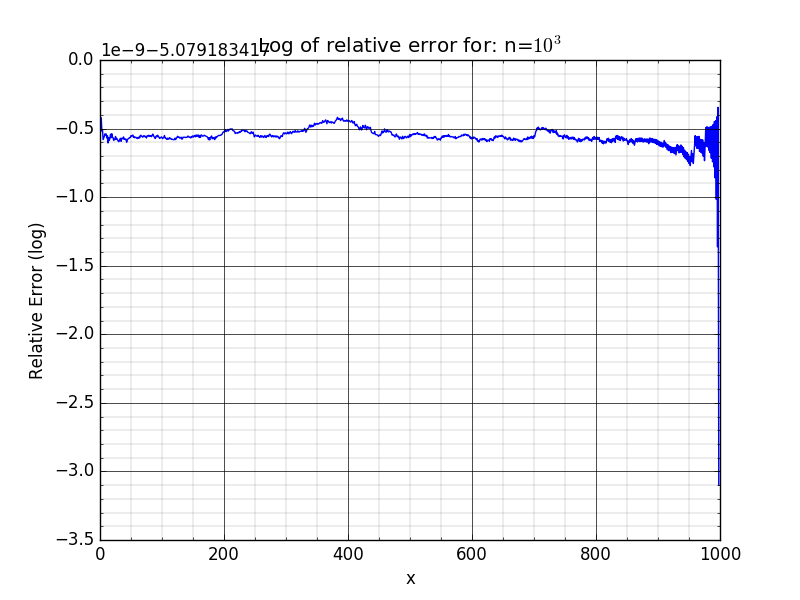
\includegraphics[scale=0.22]{3_error.png}
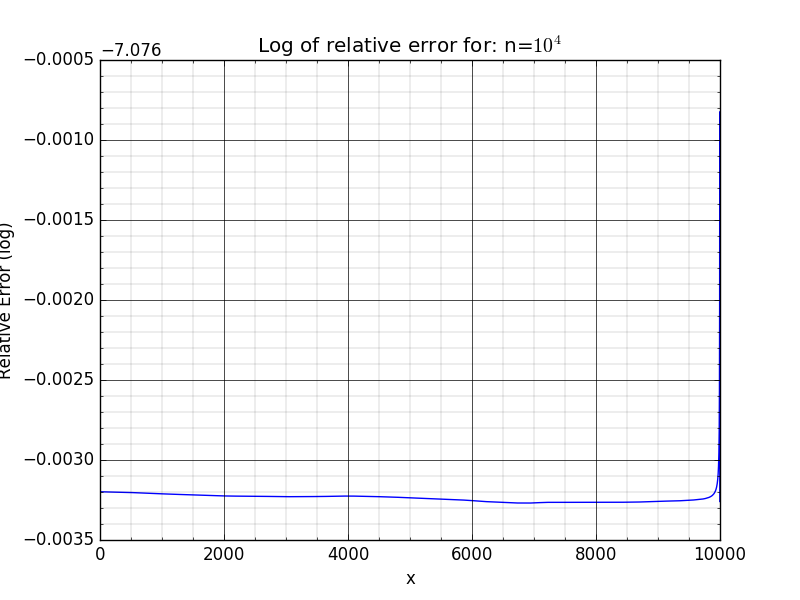
\includegraphics[scale=0.22]{4_error.png}
\centering
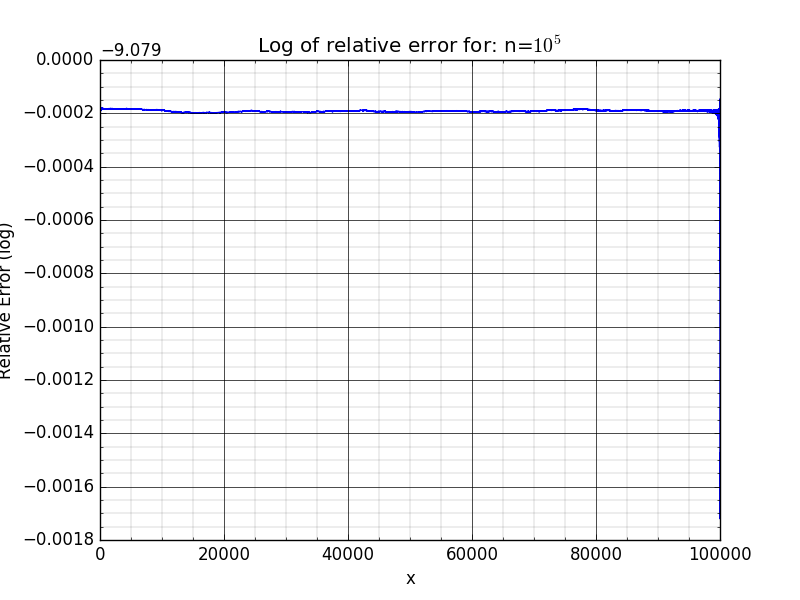
\includegraphics[scale=0.22]{5_error.png}\\
\centering
\caption{ Plots of the relative error between analytical and exact solution for numerical Gaussian elimination}
\end{figure}

Plots of the relative error between analytical and exact solution for numerical Gaussian elimination. Additionally, to verify that the algorithm was working correctly, the overall error as the solver progresses was captured and plotted since the variations in relative error can seem unintuitive. For each n, the average of the relative error is acquired. Additionally, to verify that the algorithm was working correctly, the overall error as the solver progresses was captured and plotted since the variations in relative error can seem unintuitive. For each n, the average of the relative error is acquired.\\

\begin{figure}[H]
	\centering
	\graphicspath{{~/GitHub/sayboltm/PHY480/Project1/Report/Precision/Gauss/} {c:/Users/charl/Documents/Precision/Gauss/}{C:/Users/Mike/Documents/GitHub/sayboltm/PHY480/Project1/Report/Precision/Gauss/}}
	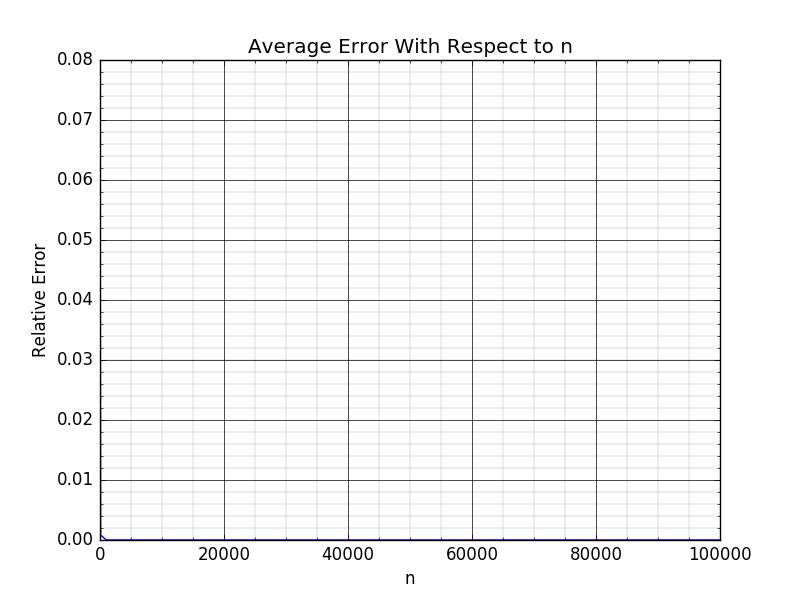
\includegraphics[scale=0.22]{BigError.png}
	\caption{Average error with respect to n for Gaussian elimination on a linear scale}
\end{figure}
 \pagebreak
As n is increased, the overall relative error decreases, which is to be expected as the approximation is closer to the exact result. It is easier to see the trend when plotted on a log scale.\\

\begin{figure}[H]
\centering
\graphicspath{{~/GitHub/sayboltm/PHY480/Project1/Report/Precision/Gauss/} {c:/Users/charl/Documents/Precision/Gauss/}{C:/Users/Mike/Documents/GitHub/sayboltm/PHY480/Project1/Report/Precision/Gauss/}}
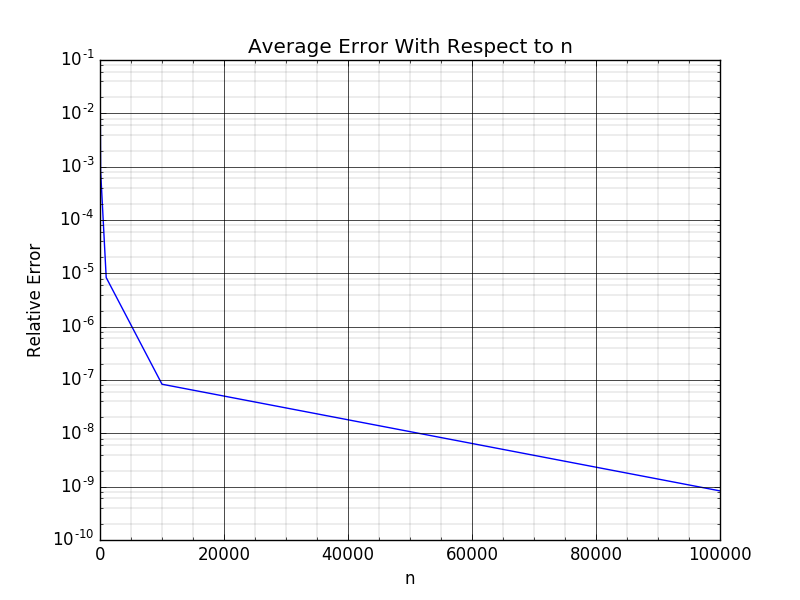
\includegraphics[scale=0.22]{BigError_log.png}
\caption{Average error with respect to n for Gaussian elimination on a log scale}
\end{figure}

\subsection{LU Decomposition:}
Figure a shows the analytical solution and the numerical solution for various n using the LU decomposition function-based solver. As n increases, the result is more tightly fit to the analytical solution which is expected.\\

\begin{figure}[H]
\centering
\graphicspath{{~/GitHub/sayboltm/PHY480/Project1/Report/Precision/LU/} {c:/Users/charl/Documents/Precision/LU/}{C:/Users/Mike/Documents/GitHub/sayboltm/PHY480/Project1/Report/Precision/LU/}}
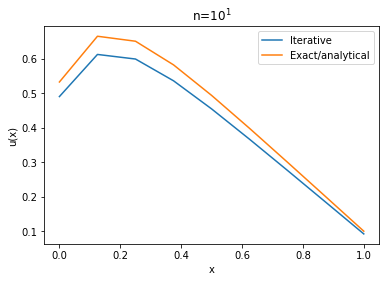
\includegraphics[scale=0.22]{1.png}
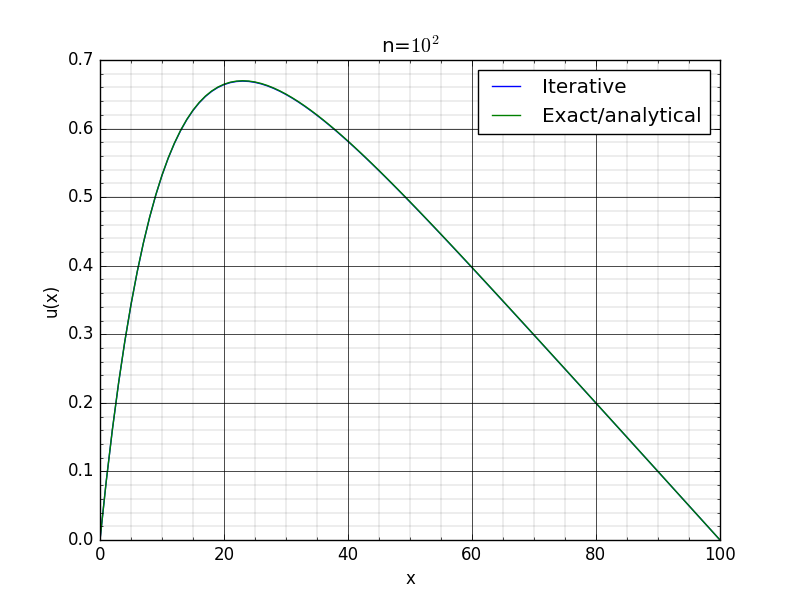
\includegraphics[scale=0.22]{2.png}
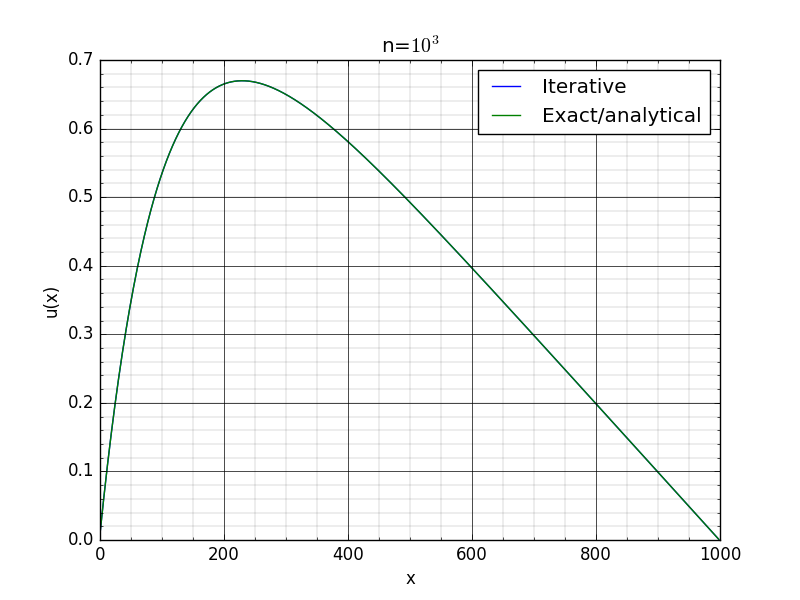
\includegraphics[scale=0.22]{3.png}
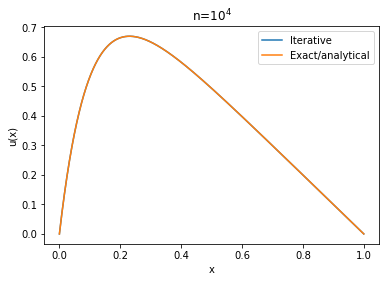
\includegraphics[scale=0.22]{4.png}\\
\centering
\caption{Plots of the analytical solution and numerical solution for solving with LU decomposition. The relative error is plotted for the LU decomposition as well in figure b.}
\end{figure}

\begin{figure}[H]
\centering
\graphicspath{{~/GitHub/sayboltm/PHY480/Project1/Report/Precision/LU/} {c:/Users/charl/Documents/Precision/LU/}{C:/Users/Mike/Documents/GitHub/sayboltm/PHY480/Project1/Report/Precision/LU/}}
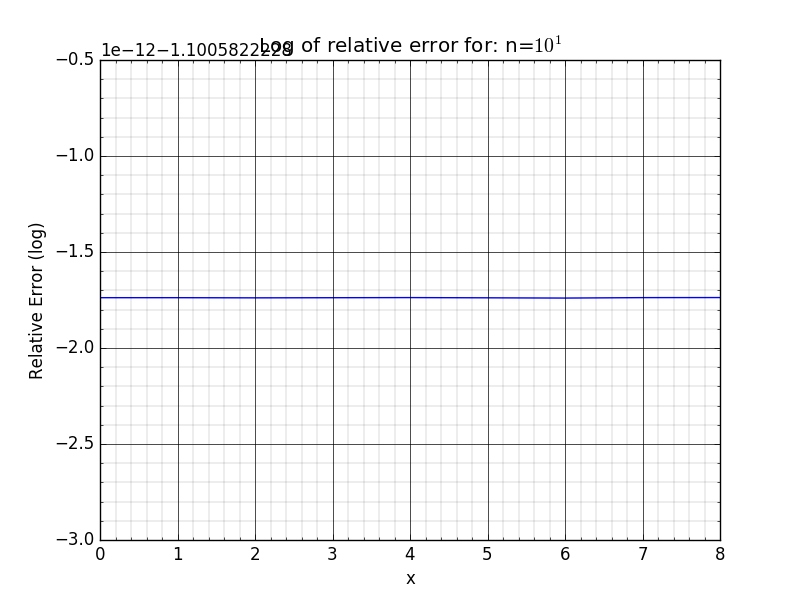
\includegraphics[scale=0.22]{1_error.png}
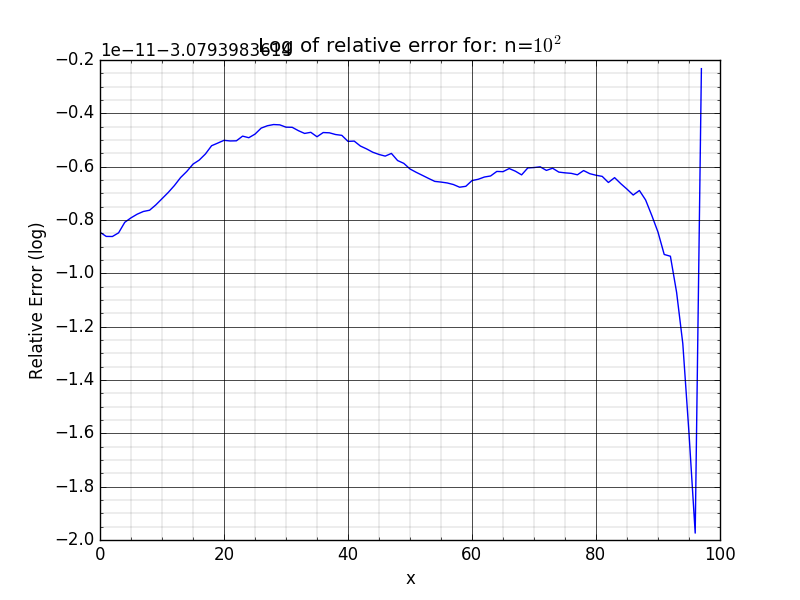
\includegraphics[scale=0.22]{2_error.png}
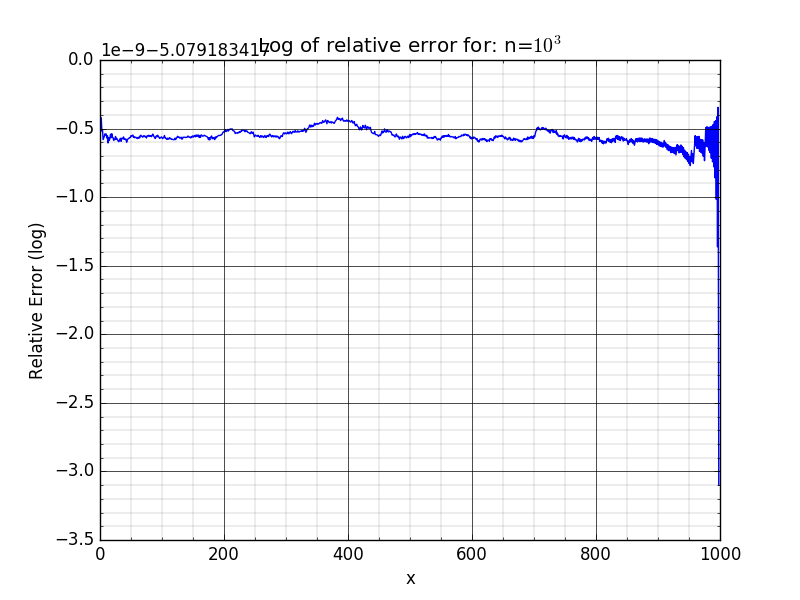
\includegraphics[scale=0.22]{3_error.png}
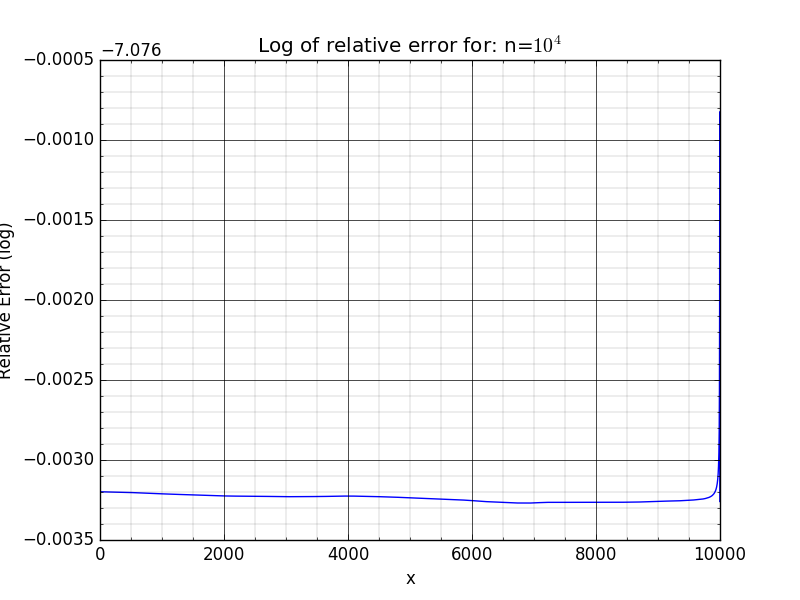
\includegraphics[scale=0.22]{4_error.png}\\
\centering
\caption{ Plots of the relative error between analytical and exact solution when solving with LU decomposition.	The overall error is also plotted, both on linear and log scales}
\end{figure}

\begin{figure}[H]
\centering
\graphicspath{{~/GitHub/sayboltm/PHY480/Project1/Report/Precision/LU/} {c:/Users/charl/Documents/Precision/LU/}{C:/Users/Mike/Documents/GitHub/sayboltm/PHY480/Project1/Report/Precision/LU/}}
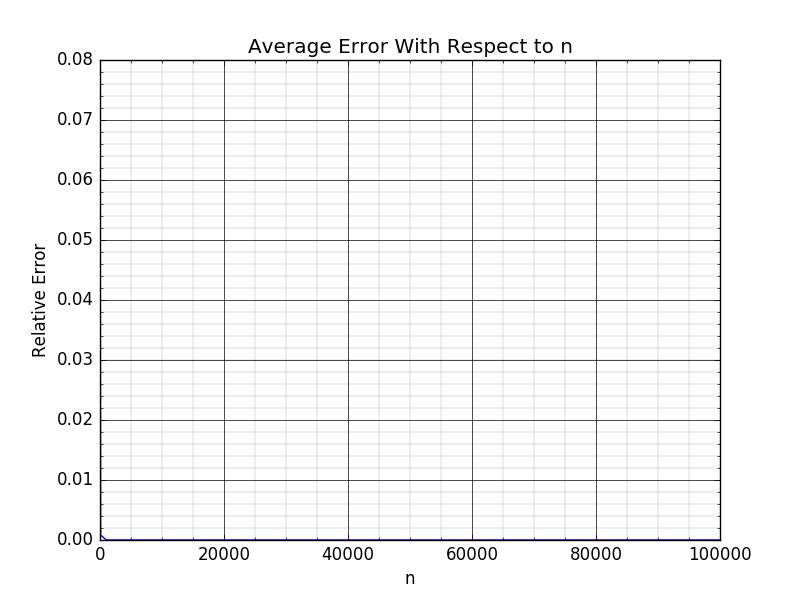
\includegraphics[scale=0.22]{BigError.png}
\caption{Average error for LU decomposition on a linear scale}
\end{figure}

\begin{figure}[H]
\centering
\graphicspath{{~/GitHub/sayboltm/PHY480/Project1/Report/Precision/LU/} {c:/Users/charl/Documents/Precision/LU/}{C:/Users/Mike/Documents/GitHub/sayboltm/PHY480/Project1/Report/Precision/LU/}}
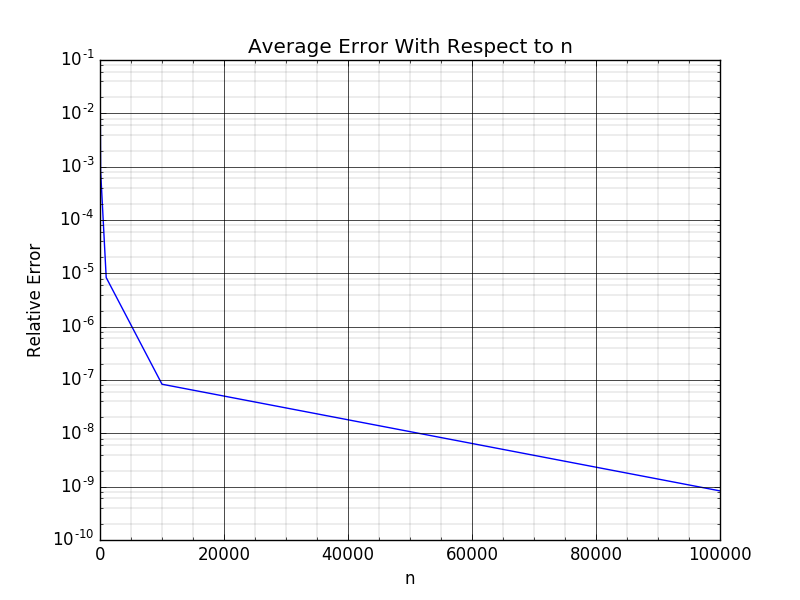
\includegraphics[scale=0.22]{BigError_log.png}
\caption{Average error for LU decomposition on a log scale}
\end{figure}

Interestingly enough, the LU decomposition could only go to $n=10^4$ before running out of memory instead of $n=10^5$ for the Gaussian elimination solver. Perhaps the implementation in the $Numpy$ library does not allocate memory well.


\subsection{Speed of Execution}
Each method that has been utilized to solve the original equation has been timed using the $date.now()$ functionality in Python. The fastest method was the General Gauss Elimination while LU Decomposition was lagging behind it. While I was definitely limited by my computing power I believe that these times could be reproduced by any other computer with reasonable computer power. The LU Decomposition was an average of 10 times slower than the General Solver.\\
\begin{table}[H]
	\centering
	\bigskip
	\bigskip
	\bigskip
	
	\begin{tabular}{l|l|l|l|l|}
		& n = 2    & n = 3    & n = 4    & n = 5    \\ \hline
		LU Decomposition  & 0.001441 & 0.014482 & 0.12671  & 54.6002  \\ \hline
		Gauss Elimination & 0.008974 & 0.063471 & 0.575171 & 5.686529 \\ \hline
	\end{tabular}
	\caption{This chart shows how the average time for each method}
\end{table}
The chart shows the average time for each method run ten (10) times. At $n < 5$ the LU Decomposition no longer is of the same magnitude, but it 10 times larger than the average times of the Gauss Elimination. 
\pagebreak
\section{Conclusions}
From examining all of the methods used to solve the original linear equation we have concluded that the Gauss Elimination method is the most efficient at finding our solution, followed by the LU Decomposition. Lastly the least efficient method used to solve the linear equation was the LU Decomposition Solver.
\section{References}
\begin{itemize}
	\item  Hjort-Jensen, M., 2015. Computational physics. \\$https://github.com/CompPhysics/ComputationalPhysics/$
\end{itemize}

\end{document}
